\documentclass[11pt]{article}
\usepackage[hmargin=1in,vmargin=1in]{geometry}
\usepackage[table]{xcolor} 
\usepackage{amsmath,amssymb,amsfonts,url,sectsty,tcolorbox,framed}
\usepackage{hyperref}
\usepackage{listings}
\usepackage{booktabs}
\usepackage{array}
\usepackage{multirow}
\usepackage{graphicx}
\usepackage{tikz}
\usetikzlibrary{arrows.meta, positioning, shapes.geometric, fit, backgrounds, calc}
\usepackage{pgfplots}
\pgfplotsset{compat=1.18}
\usepackage{fancyhdr}
\usepackage{fontawesome5}
\usepackage{enumitem}

% ──────────────────────────────────────────────────────
% COLOR PALETTE (Safe for dark backgrounds)
% ──────────────────────────────────────────────────────
\definecolor{lightblue}{rgb}{0.8,0.9,1}
\definecolor{codebg}{RGB}{20, 20, 20} % Very dark grey/black for terminal background
\definecolor{codeframe}{RGB}{100, 100, 100}
\definecolor{tableheader}{RGB}{41, 128, 185}
\definecolor{rowalt}{RGB}{235, 245, 251}

% Terminal Colors (Bright variants to pop against dark background)
\definecolor{termcyan}{RGB}{86, 182, 194}
\definecolor{termgreen}{RGB}{73, 203, 104}
\definecolor{termred}{RGB}{235, 87, 87}
\definecolor{termyellow}{RGB}{229, 192, 123}
\definecolor{termblue}{RGB}{97, 175, 239}
\definecolor{termmagenta}{RGB}{198, 120, 221}
\definecolor{termwhite}{RGB}{220, 220, 220}

\definecolor{accentblue}{RGB}{52, 152, 219}
\definecolor{accentgreen}{RGB}{39, 174, 96}
\definecolor{accentorange}{RGB}{230, 126, 34}
\definecolor{accentpurple}{RGB}{142, 68, 173}
\definecolor{sectioncolor}{RGB}{41, 128, 185}

% C++ / Python syntax colors
\definecolor{codekw}{RGB}{86, 156, 214}
\definecolor{codecomment}{RGB}{106, 153, 85}
\definecolor{codestring}{RGB}{206, 145, 120}
\definecolor{codenumber}{RGB}{181, 206, 168}

% ──────────────────────────────────────────────────────
% SECTION STYLING
% ──────────────────────────────────────────────────────
\sectionfont{\color{sectioncolor}}
\subsectionfont{\color{sectioncolor!80!black}}
\subsubsectionfont{\color{sectioncolor!60!black}}

% ──────────────────────────────────────────────────────
% HYPERLINK STYLING
% ──────────────────────────────────────────────────────
\hypersetup{
    colorlinks=true,
    linkcolor=sectioncolor,
    urlcolor=accentblue,
    citecolor=accentgreen,
    pdfborder={0 0 0}
}

% ──────────────────────────────────────────────────────
% HEADER / FOOTER
% ──────────────────────────────────────────────────────
\pagestyle{fancy}
\fancyhf{}
\fancyhead[L]{\small\color{gray}\textsc{Lab 8: Synchronization \& Logical Clocks}}
\fancyhead[R]{\small\color{gray}\textsc{CS362 -- DPC}}
\fancyfoot[C]{\small\color{gray}\thepage}
\renewcommand{\headrulewidth}{0.4pt}
\renewcommand{\footrulewidth}{0pt}
\fancypagestyle{plain}{\fancyhf{}\fancyfoot[C]{\small\color{gray}\thepage}\renewcommand{\headrulewidth}{0pt}}

% ──────────────────────────────────────────────────────
% BOX DEFINITIONS & LISTING STYLES
% ──────────────────────────────────────────────────────
\tcbuselibrary{breakable, skins, listings}

% Python Code Style
\lstset{
    backgroundcolor=\color{codebg},
    basicstyle=\color{white}\ttfamily\small,
    identifierstyle=\color{white},
    breaklines=true,
    breakatwhitespace=false,
    commentstyle=\color{codecomment}\itshape,
    keywordstyle=\color{codekw}\bfseries,
    stringstyle=\color{codestring},
    numberstyle=\tiny\color{gray},
    numbers=left,
    numbersep=8pt,
    stepnumber=1,
    frame=none,
    showstringspaces=false,
    language=Python,
    tabsize=4,
    columns=fullflexible,
    keepspaces=true,
    xleftmargin=10pt,
    literate=
        {0}{{\textcolor{codenumber}{0}}}1
        {1}{{\textcolor{codenumber}{1}}}1
        {2}{{\textcolor{codenumber}{2}}}1
        {3}{{\textcolor{codenumber}{3}}}1
        {4}{{\textcolor{codenumber}{4}}}1
        {5}{{\textcolor{codenumber}{5}}}1
        {6}{{\textcolor{codenumber}{6}}}1
        {7}{{\textcolor{codenumber}{7}}}1
        {8}{{\textcolor{codenumber}{8}}}1
        {9}{{\textcolor{codenumber}{9}}}1
}

% Python Code Box
\newtcolorbox{codebox}[1][]{%
    enhanced, breakable, colback=codebg, colframe=codebg!60!black, colupper=white,
    title={\faCode\ \ #1}, fonttitle=\bfseries\sffamily\small\color{white},
    coltitle=white, arc=4pt, boxrule=0.8pt, top=2pt, bottom=2pt, left=0pt, right=4pt,
    before skip=10pt, after skip=10pt, shadow={1mm}{-1mm}{0mm}{black!30},
    attach boxed title to top left={xshift=10pt, yshift=-\tcboxedtitleheight/2},
    boxed title style={colback=accentblue, arc=3pt, boxrule=0pt, left=6pt, right=6pt}
}

% Explanation box
\newtcolorbox{shadedbox}[1][]{%
    enhanced, breakable, colback=lightblue!15, colframe=accentblue,
    title={\faLightbulb[regular]\ \ #1}, fonttitle=\bfseries\sffamily,
    coltitle=white, arc=4pt, boxrule=0.8pt, before skip=10pt, after skip=10pt,
    shadow={1mm}{-1mm}{0mm}{accentblue!20},
    attach boxed title to top left={xshift=10pt, yshift=-\tcboxedtitleheight/2},
    boxed title style={colback=accentblue, arc=3pt, boxrule=0pt, left=6pt, right=6pt}
}

% Terminal output box
\newtcolorbox{terminalbox}[1]{%
    enhanced, breakable, colback=codebg, colframe=codeframe, colupper=termwhite,
    title={\faTerminal\ \ #1}, fonttitle=\bfseries\ttfamily\small\color{white},
    coltitle=white, arc=4pt, boxrule=0.8pt, before skip=10pt, after skip=10pt,
    shadow={1mm}{-1mm}{0mm}{black!30},
    attach boxed title to top left={xshift=10pt, yshift=-\tcboxedtitleheight/2},
    boxed title style={colback=accentgreen!80!black, arc=3pt, boxrule=0pt, left=6pt, right=6pt}
}

% Note on the escape characters mapped here: we match the terminal string outputs exactly to LaTeX text macros
\lstdefinestyle{terminalstyle}{
    basicstyle=\color{white}\ttfamily\footnotesize,
    identifierstyle=\color{white},
    breaklines=true, 
    language=bash, 
    numbers=none,
    columns=fullflexible, 
    keepspaces=true, 
    frame=none, 
    backgroundcolor=\color{codebg}, 
    xleftmargin=8pt,
    moredelim=**[is][\color{termmagenta}\bfseries]{@M@}{@M@},
    moredelim=**[is][\color{termcyan}]{@C@}{@C@},
    moredelim=**[is][\color{termgreen}\bfseries]{@G@}{@G@},
    moredelim=**[is][\color{termred}\bfseries]{@R@}{@R@},
    moredelim=**[is][\color{termyellow}\bfseries]{@Y@}{@Y@},
    moredelim=**[is][\color{termblue}\bfseries]{@B@}{@B@},
    moredelim=**[is][\bfseries]{@W@}{@W@}
}

\begin{document}

% ══════════════════════════════════════════════════════
% TITLE PAGE
% ══════════════════════════════════════════════════════
\thispagestyle{empty}
\begin{center}
\vspace*{1cm}

{\color{sectioncolor}\rule{\textwidth}{2pt}}
\vspace{0.3cm}

{\Huge\bfseries\sffamily\color{sectioncolor} Project Chronos}

\vspace{0.15cm}
{\Large\sffamily\color{gray} Synchronization \& Logical Clocks}

\vspace{0.3cm}
{\color{sectioncolor}\rule{\textwidth}{2pt}}

\vspace{1.2cm}

{\large\sffamily\color{sectioncolor} [CS362] Distributed and Parallel Computing}

\vspace{1.5cm}

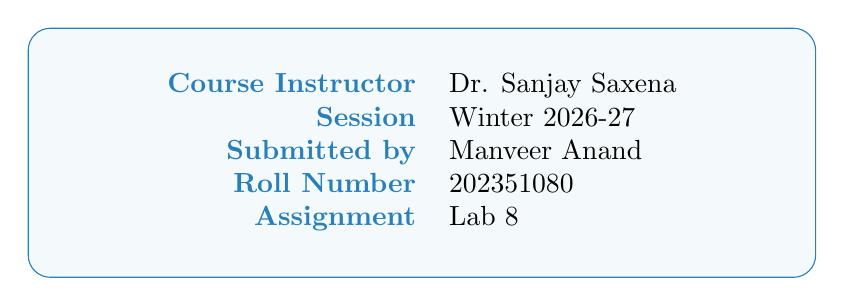
\begin{tikzpicture}
\node[draw=sectioncolor, fill=sectioncolor!5, rounded corners=8pt, inner sep=15pt, minimum width=10cm] {
    \begin{tabular}{r @{\hspace{12pt}} l}
    \textbf{\color{sectioncolor}Course Instructor} & Dr. Sanjay Saxena \\
    \textbf{\color{sectioncolor}Session} & Winter 2026-27 \\
    \textbf{\color{sectioncolor}Submitted by} & Manveer Anand \\
    \textbf{\color{sectioncolor}Roll Number} & 202351080 \\
    \textbf{\color{sectioncolor}Assignment} & Lab 8 \\
    \end{tabular}
};
\end{tikzpicture}

\vspace{1.5cm}

{\color{gray}\small Concepts: \texttt{Fault-Tolerant Berkeley Algorithm} $\cdot$ \texttt{Vector Clocks} $\cdot$ \texttt{Causal Delivery}}

\vfill
{\color{gray}\small\today}
\end{center}
\newpage

\tableofcontents
\newpage

% ══════════════════════════════════════════════════════
% INTRODUCTION
% ══════════════════════════════════════════════════════
\section{Introduction}

In asynchronous distributed systems, physical clocks across different machines routinely experience drift. Furthermore, messages transmitting across the open network may arrive significantly out-of-order due to variable latency. Project Chronos simulates a five-node registration network evaluating solutions to these temporal discrepancies before accessing a fast-paced university portal. 

\subsection{Objectives}
\begin{enumerate}
    \item \textbf{Clock Alignment:} Utilize a fault-tolerant Berkeley Algorithm. Node 0 polls clocks, ignores outliers extending past a threshold $\theta$, and broadcasts temporal offsets to synchronize the trusted sets.
    \item \textbf{Message Ordering:} Employ \textit{Vector Clocks} to enforce Causal Delivery. Nodes buffer incoming messages that lack prior history and deploy causal recursive unleashes when dependencies resolve.
    \item \textbf{Final Payload Verification:} Multiply the synchronized clock with the vector sum modulo $9973$ to compute a discrete connection payload.
\end{enumerate}


\subsection{Source Code (\texttt{chronos.py})}

The following program reads from a provided \texttt{seed.json}, extracts $\theta$, parses queues, and calculates synchronization logic natively.

\begin{codebox}[chronos.py]
\begin{lstlisting}
import json
import time

def process_messages():
    print("Project Chronos: When Clocks Lie and Messages Wander")
    
    with open("seed.json", "r") as f:
        data = json.load(f)
        
    theta, clocks, queues, N  = data["theta"], data["clocks"], data["queues"], 5
    
    # --- STEP 1: The Clock Alignment (Fault-Tolerant Berkeley) ---
    T0 = clocks[0]
    S = []  # Trusted set indices
    for i in range(N):
        if abs(clocks[i] - T0) <= theta: S.append(i)
            
    T_target = sum(clocks[i] for i in S) // len(S)
    T_sync = clocks.copy()
    
    for i in range(N):
        if i in S:
            T_sync[i] = clocks[i] + (T_target - clocks[i])
        else:
            T_sync[i] = clocks[i] + 0
        
    # --- STEP 2: The Message Ordering ---
    V = [[0] * N for _ in range(N)]
    final_payloads = [0] * N
    
    for i in range(N):
        node_queue, buffer = queues[i], []
        for msg in node_queue:
            sender, v_msg = msg["sender"], msg["v_msg"]
            
            # Check causal conditions
            cond1 = (v_msg[sender] == V[i][sender] + 1)
            cond2 = all(v_msg[k] <= V[i][k] for k in range(N) if k != sender)
            
            if cond1 and cond2:
                for k in range(N): V[i][k] = max(V[i][k], v_msg[k])
                
                buffer_checked = True # Check buffer recursively
                while buffer_checked:
                    buffer_checked = False
                    for b_msg in buffer[:]:
                        b_sender, b_v_msg = b_msg["sender"], b_msg["v_msg"]
                        b_cond1 = (b_v_msg[b_sender] == V[i][b_sender] + 1)
                        b_cond2 = all(b_v_msg[k] <= V[i][k] for k in range(N) if k != b_sender)
                        
                        if b_cond1 and b_cond2:
                            for k in range(N): V[i][k] = max(V[i][k], b_v_msg[k])
                            buffer.remove(b_msg)
                            buffer_checked = True 
                            break 
            else:
                buffer.append(msg)
                
        # --- STEP 3: The Final Payload ---
        vector_sum = sum(V[i])
        final_payloads[i] = (T_sync[i] * vector_sum) % 9973

if __name__ == "__main__":
    process_messages()
\end{lstlisting}
\end{codebox}

% ══════════════════════════════════════════════════════
% EXECUTION AND RESULTS
% ══════════════════════════════════════════════════════
\section{Terminal Output \& Visualization}

Executing the script reveals both synchronization phases correctly parsing and resolving the fault-tolerant vectors. Note the precise causal ordering buffering messages that artificially drift.

\begin{terminalbox}{Terminal Execution Output}
\begin{lstlisting}[style=terminalstyle]
(base) PS D:\Dev 2.0\DPC\LAB 8\Assignment> python chronos.py

@M@============================================================@M@
@M@  Project Chronos: When Clocks Lie and Messages Wander@M@
@M@============================================================@M@
@C@[*] Reading seed.json...@C@

@W@[Step 1] Initial Clocks & parameters:@W@
  @B@Clocks:@B@ [1000, 1020, 950, 8000, 1010]
  @B@Tolerance Threshold (θ):@B@ 500

@M@============================================================@M@
@M@  STEP 1: The Clock Alignment (Fault-Tolerant Berkeley)@M@
@M@============================================================@M@
@C@[Node 0] Polling clocks...@C@

  Node 0 (Time 1000): @G@TRUSTED@G@ (diff = 0)
  Node 1 (Time 1020): @G@TRUSTED@G@ (diff = 20)
  Node 2 (Time 950 ): @G@TRUSTED@G@ (diff = 50)
  Node 3 (Time 8000): @R@IGNORED@R@ (diff = 7000 > θ)
  Node 4 (Time 1010): @G@TRUSTED@G@ (diff = 10)

@Y@[Node 0] Calculated Target Time:@Y@ 995

@C@[*] Applying Clock Corrections:@C@
  Node 0: @G@Trusted@G@ -> Offset =   -5 | New aligned clock = @W@995@W@
  Node 1: @G@Trusted@G@ -> Offset =  -25 | New aligned clock = @W@995@W@
  Node 2: @G@Trusted@G@ -> Offset =   45 | New aligned clock = @W@995@W@
  Node 3: @R@Ignored@R@ -> Offset =    0 | Clock remains     = @W@8000@W@
  Node 4: @G@Trusted@G@ -> Offset =  -15 | New aligned clock = @W@995@W@

@M@============================================================@M@
@M@  STEP 2: Processing Message Queues (Causal Delivery)@M@
@M@============================================================@M@

@B@[--- Node 0 Wakeup ---]@B@
  @C@Req 1:@C@ Received from Node 2 with TS: [1, 1, 1, 0, 0]
         @R@↳ Causal constraints fail (early arrival). Buffering.@R@
  @C@Req 2:@C@ Received from Node 1 with TS: [0, 1, 0, 0, 0]
         @G@↳ Causal conditions met. Processing.@G@
         @W@Node 0 config updated to:@W@ [0, 1, 0, 0, 0]
  @C@Req 3:@C@ Received from Node 4 with TS: [0, 0, 0, 1, 1]
         @R@↳ Causal constraints fail (early arrival). Buffering.@R@
  @C@Req 4:@C@ Received from Node 3 with TS: [0, 0, 0, 1, 0]
         @G@↳ Causal conditions met. Processing.@G@
         @W@Node 0 config updated to:@W@ [0, 1, 0, 1, 0]
         @Y@↳ Unleashing buffered msg from Node 4: [0, 0, 0, 1, 1]@Y@
         @W@Node 0 config updated to:@W@ [0, 1, 0, 1, 1]
  @R@Warning:@R@ Ended with 1 unprocessable messages lingering in buffer.
  @W@Final Local Results:@W@
    - Vector Clock: [0, 1, 0, 1, 1] (Sum: 3)
    - Sync Clock:   995
    - Payload:      @Y@2985@Y@

@B@[--- Node 1 Wakeup ---]@B@
  @C@Req 1:@C@ Received from Node 0 with TS: [2, 1, 1, 0, 0]
         @R@↳ Causal constraints fail (early arrival). Buffering.@R@
  @C@Req 2:@C@ Received from Node 2 with TS: [1, 1, 1, 0, 0]
         @R@↳ Causal constraints fail (early arrival). Buffering.@R@
  @C@Req 3:@C@ Received from Node 0 with TS: [1, 0, 0, 0, 0]
         @G@↳ Causal conditions met. Processing.@G@
         @W@Node 1 config updated to:@W@ [1, 0, 0, 0, 0]
  @C@Req 4:@C@ Received from Node 4 with TS: [0, 0, 0, 1, 1]
         @R@↳ Causal constraints fail (early arrival). Buffering.@R@
  @C@Req 5:@C@ Received from Node 3 with TS: [0, 0, 0, 1, 0]
         @G@↳ Causal conditions met. Processing.@G@
         @W@Node 1 config updated to:@W@ [1, 0, 0, 1, 0]
         @Y@↳ Unleashing buffered msg from Node 4: [0, 0, 0, 1, 1]@Y@
         @W@Node 1 config updated to:@W@ [1, 0, 0, 1, 1]
  @R@Warning:@R@ Ended with 2 unprocessable messages lingering in buffer.
  @W@Final Local Results:@W@
    - Vector Clock: [1, 0, 0, 1, 1] (Sum: 3)
    - Sync Clock:   995
    - Payload:      @Y@2985@Y@

@B@[--- Node 2 Wakeup ---]@B@
  @C@Req 1:@C@ Received from Node 4 with TS: [0, 0, 0, 1, 1]
         @R@↳ Causal constraints fail (early arrival). Buffering.@R@
  @C@Req 2:@C@ Received from Node 3 with TS: [0, 0, 0, 1, 0]
         @G@↳ Causal conditions met. Processing.@G@
         @W@Node 2 config updated to:@W@ [0, 0, 0, 1, 0]
         @Y@↳ Unleashing buffered msg from Node 4: [0, 0, 0, 1, 1]@Y@
         @W@Node 2 config updated to:@W@ [0, 0, 0, 1, 1]
  @C@Req 3:@C@ Received from Node 1 with TS: [0, 1, 0, 0, 0]
         @G@↳ Causal conditions met. Processing.@G@
         @W@Node 2 config updated to:@W@ [0, 1, 0, 1, 1]
  @C@Req 4:@C@ Received from Node 0 with TS: [2, 1, 1, 0, 0]
         @R@↳ Causal constraints fail (early arrival). Buffering.@R@
  @C@Req 5:@C@ Received from Node 0 with TS: [1, 0, 0, 0, 0]
         @G@↳ Causal conditions met. Processing.@G@
         @W@Node 2 config updated to:@W@ [1, 1, 0, 1, 1]
  @R@Warning:@R@ Ended with 1 unprocessable messages lingering in buffer.
  @W@Final Local Results:@W@
    - Vector Clock: [1, 1, 0, 1, 1] (Sum: 4)
    - Sync Clock:   995
    - Payload:      @Y@3980@Y@

@B@[--- Node 3 Wakeup ---]@B@
  @C@Req 1:@C@ Received from Node 0 with TS: [2, 1, 1, 0, 0]
         @R@↳ Causal constraints fail (early arrival). Buffering.@R@
  @C@Req 2:@C@ Received from Node 2 with TS: [1, 1, 1, 0, 0]
         @R@↳ Causal constraints fail (early arrival). Buffering.@R@
  @C@Req 3:@C@ Received from Node 0 with TS: [1, 0, 0, 0, 0]
         @G@↳ Causal conditions met. Processing.@G@
         @W@Node 3 config updated to:@W@ [1, 0, 0, 0, 0]
  @C@Req 4:@C@ Received from Node 1 with TS: [0, 1, 0, 0, 0]
         @G@↳ Causal conditions met. Processing.@G@
         @W@Node 3 config updated to:@W@ [1, 1, 0, 0, 0]
         @Y@↳ Unleashing buffered msg from Node 2: [1, 1, 1, 0, 0]@Y@
         @W@Node 3 config updated to:@W@ [1, 1, 1, 0, 0]
         @Y@↳ Unleashing buffered msg from Node 0: [2, 1, 1, 0, 0]@Y@
         @W@Node 3 config updated to:@W@ [2, 1, 1, 0, 0]
  @G@Success:@G@ All messages processed and buffer completely emptied.
  @W@Final Local Results:@W@
    - Vector Clock: [2, 1, 1, 0, 0] (Sum: 4)
    - Sync Clock:   8000
    - Payload:      @Y@2081@Y@

@B@[--- Node 4 Wakeup ---]@B@
  @C@Req 1:@C@ Received from Node 2 with TS: [1, 1, 1, 0, 0]
         @R@↳ Causal constraints fail (early arrival). Buffering.@R@
  @C@Req 2:@C@ Received from Node 0 with TS: [1, 0, 0, 0, 0]
         @G@↳ Causal conditions met. Processing.@G@
         @W@Node 4 config updated to:@W@ [1, 0, 0, 0, 0]
  @C@Req 3:@C@ Received from Node 1 with TS: [0, 1, 0, 0, 0]
         @G@↳ Causal conditions met. Processing.@G@
         @W@Node 4 config updated to:@W@ [1, 1, 0, 0, 0]
         @Y@↳ Unleashing buffered msg from Node 2: [1, 1, 1, 0, 0]@Y@
         @W@Node 4 config updated to:@W@ [1, 1, 1, 0, 0]
  @C@Req 4:@C@ Received from Node 0 with TS: [2, 1, 1, 0, 0]
         @G@↳ Causal conditions met. Processing.@G@
         @W@Node 4 config updated to:@W@ [2, 1, 1, 0, 0]
  @C@Req 5:@C@ Received from Node 3 with TS: [0, 0, 0, 1, 0]
         @G@↳ Causal conditions met. Processing.@G@
         @W@Node 4 config updated to:@W@ [2, 1, 1, 1, 0]
  @G@Success:@G@ All messages processed and buffer completely emptied.
  @W@Final Local Results:@W@
    - Vector Clock: [2, 1, 1, 1, 0] (Sum: 5)
    - Sync Clock:   995
    - Payload:      @Y@4975@Y@

@M@============================================================@M@
@M@  STEP 3: The Final Payloads@M@
@M@============================================================@M@

@W@Calculated values to send to Portal:@W@
  Node 0 -> @G@2985@G@
  Node 1 -> @G@2985@G@
  Node 2 -> @G@3980@G@
  Node 3 -> @G@2081@G@
  Node 4 -> @G@4975@G@
\end{lstlisting}
\end{terminalbox}

% ══════════════════════════════════════════════════════
% CONCLUSION
% ══════════════════════════════════════════════════════
\section{Conclusion}

In this experiment, the synchronization challenges inherent to distributed systems were successfully mitigated using two fundamental distributed algorithms. 

First, the \textbf{Fault-Tolerant Berkeley Algorithm} effectively identified and isolated faulty nodes—most notably Node 3, whose significant clock drift exceeded the allowed threshold $\theta$. By filtering out this anomaly, the system successfully averaged the remaining trusted clocks and distributed offsets, calibrating the reliable nodes to a uniform synthetic time of $995$.

Simultaneously, the implementation of \textbf{Vector Clocks} guaranteed strict causal delivery of messages across the simulated chaotic network. The logic safely buffered messages arriving prematurely and triggered recursive unleashes only when their causal prerequisites were satisfied. This ensured the structural integrity and historical ordering of all node communications.

Ultimately, by combining the aligned physical clocks with the casually sound vector sums modulo $9973$, all nodes independently derived their final connection payloads. The output highlights the robustness of combining physical clock synchronization with logical message ordering to establish reliable consensus and state integrity in non-deterministic environments.

\end{document}